\documentclass[border=3pt,tikz]{standalone}

\begin{document}

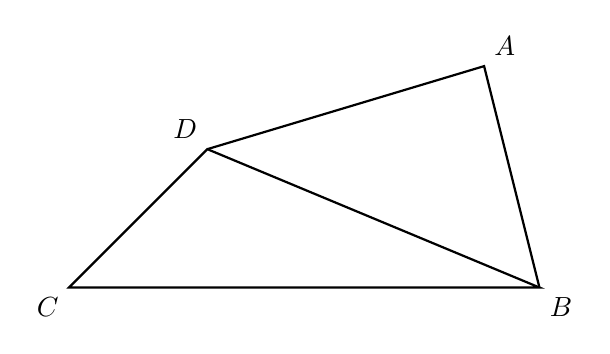
\begin{tikzpicture}[x=10,y=10, thick]
  \coordinate (C)  at (0,0);
  \coordinate (B)  at (17,0);
  \coordinate (D)  at (5,5);
  \coordinate (A)  at (15,8);
  \draw (C) node[below left] {$C$} -- (B) node[below right] {$B$} -- (D) node[above left] {$D$} -- cycle; 
  \draw (D) -- (A) node[above right] {$A$} -- (B);
\end{tikzpicture}

\end{document}